\documentclass[11pt]{article}
\usepackage[T1]{fontenc}
\usepackage[utf8]{inputenc}
\usepackage{lmodern,amsmath,amssymb,graphicx,geometry,microtype,setspace,booktabs,caption}
\usepackage[hidelinks]{hyperref}
\geometry{letterpaper,margin=1in}
\setlength{\parindent}{0pt}
\setlength{\parskip}{0.55em}
\setlength{\emergencystretch}{2em}
\captionsetup{labelfont=bf,font=small}
\renewcommand{\refname}{References}
\pagestyle{empty}
\renewcommand{\thefigure}{S\arabic{figure}}
\setcounter{figure}{15}
\begin{document}
\begin{figure}[!ht]\centering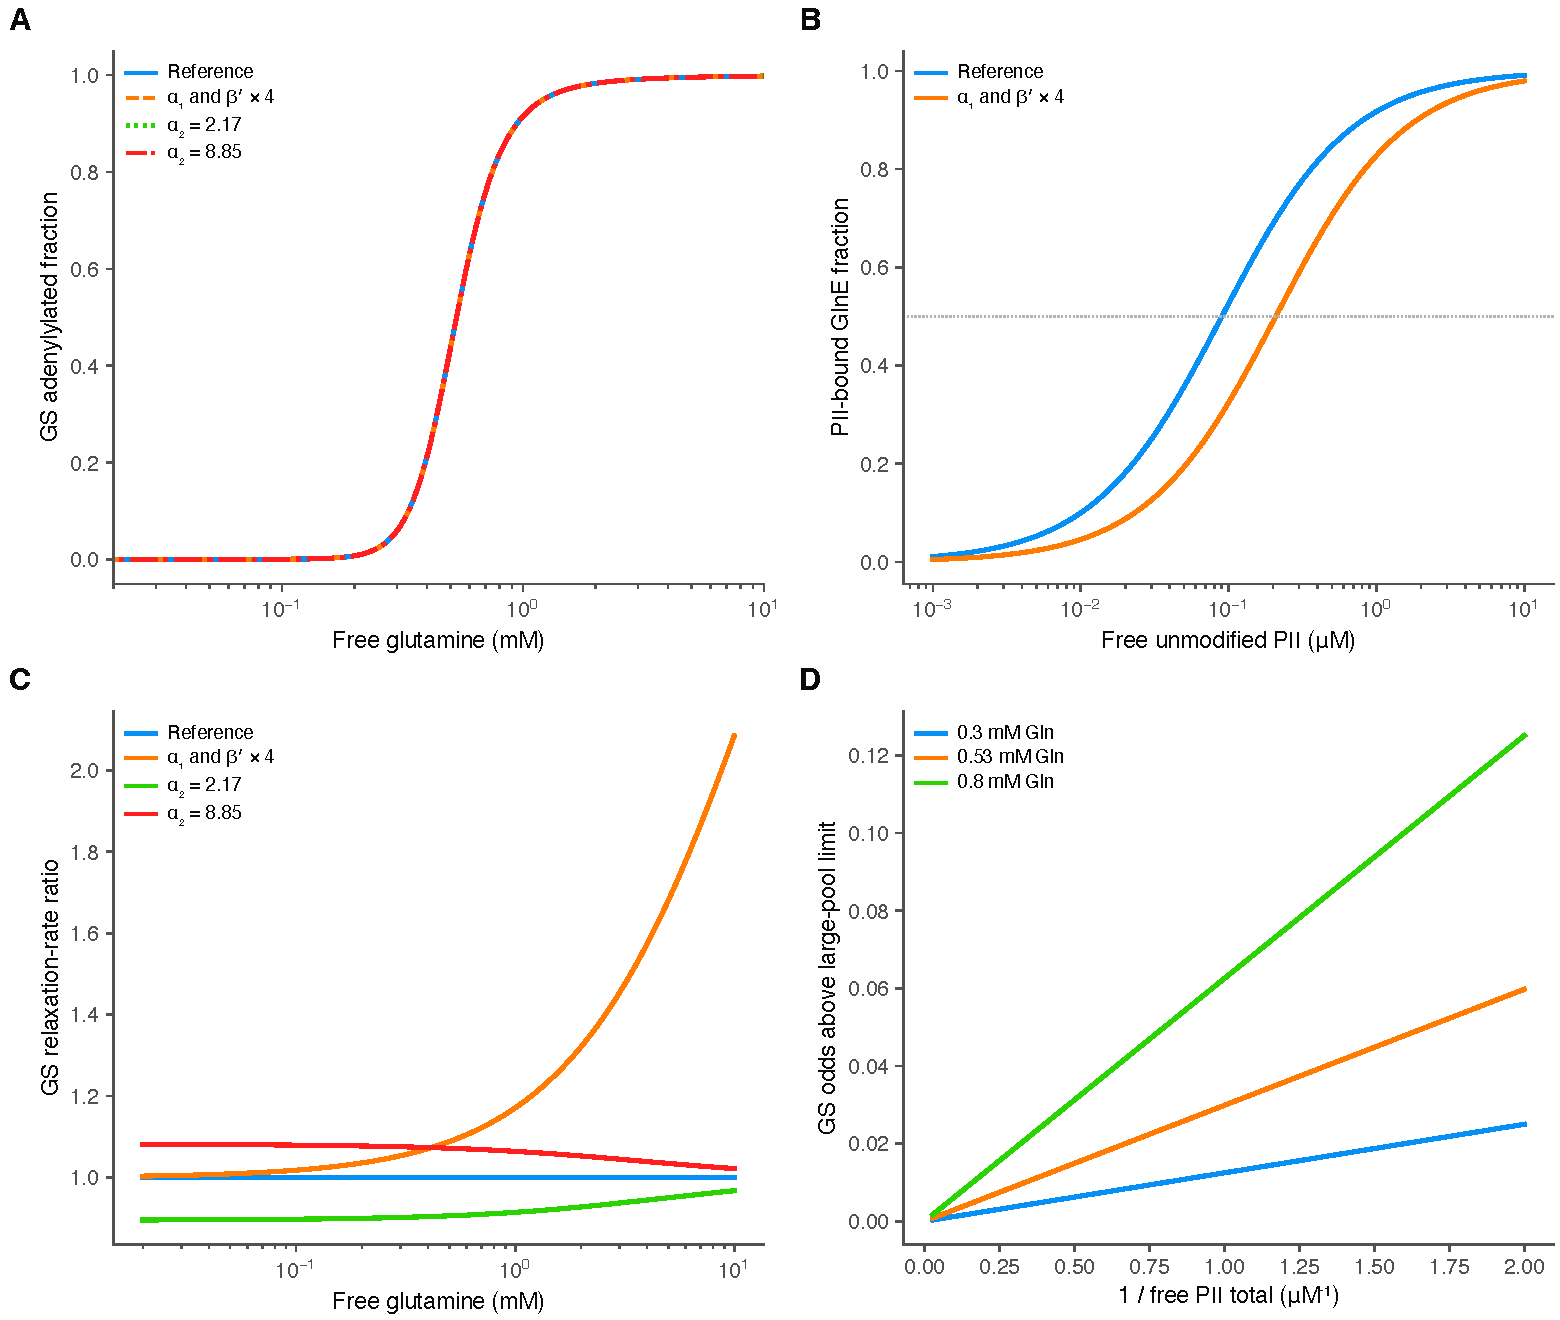
\includegraphics[width=\textwidth,height=0.60\textheight,keepaspectratio]{figure_inputs/FigS16_extended.pdf}\caption{\textbf{Binding and catalytic regulation in the published six-state GlnE topology.} (A) Coupled GS steady-state curves are identical after a shared binding/catalysis transformation or a change in the PII--PII-UMP interaction parameter. One reference gain sets $Y=0.5$ at 0.53 mM glutamine and $T=5\,\mu$M; it is unchanged in every variant. (B) PII-binding isotherms at fixed $G=10$ mM and $U=0.3\,\mu$M distinguish binding from catalytic synergy. (C) Reduced GS relaxation rates at separately controlled $P=1\,\mu$M and $U=0.3\,\mu$M differ along a glutamine titration. These are not the coupled inputs in A. (D) The PII-independent route gives a drive affine in inverse free-target total at fixed glutamine and modification fraction. Its analytic large-pool limit is subtracted to display the concentration-dependent term. Lines are predictions, not additional observations. S21 separates source-reported fitted constants from chosen parameters and states the rapid-binding and independent-GS assumptions.}


\end{figure}
\end{document}
